\section{Problem 3}

\subsection{Question}
\vspace*{10pt}
\justify 
Take the Twitter graph you generated in question \#1 and test for
male-female homophily.  For the purposes of this question you can
consider the graph as undirected (i.e., no distinction between
\enquote{follows} and \enquote{following}).  Use the twitter name (not \enquote{screen
name}; for example \enquote{Michael L. Nelson} and not \enquote{{@}phonedude\_mln})
and programatically determine if the user is male or female.  Some
sites that might be useful:\\
\\
\url{https://genderize.io/}\\
\url{https://pypi.python.org/pypi/gender-detector/0.0.4}\\
\\
Create a table of Twitter users and their likely gender.  List any 
accounts that can't be determined and remove them from the graph.\\
\\
Perform the homophily test as described in slides 11-15, Week 7.\\
\\
Does your Twitter graph exhibit gender homophily?

\subsection{Answer}
Using an example from the primary author of the D3 JavaScript library, Mike Bostok \cite{d3:bostok12}, a graph was created of Zachary's Karate Club using the pickled \cite{py:pickle} dataset found at \url{http://nexus.igraph.org/api/dataset_info?id=1&format=html}. The D3 library provides a force-directed graphing layout \cite{d3:force14}, which was used to display the graph. A transition from the initial graph, shown in Figure \ref{fig:init_graph}, to the graph after the split of the karate club, shown in Figure \ref{fig:split_graph}, was created using standard JavaScript.

\begin{figure}[h!]
\centering
\fbox{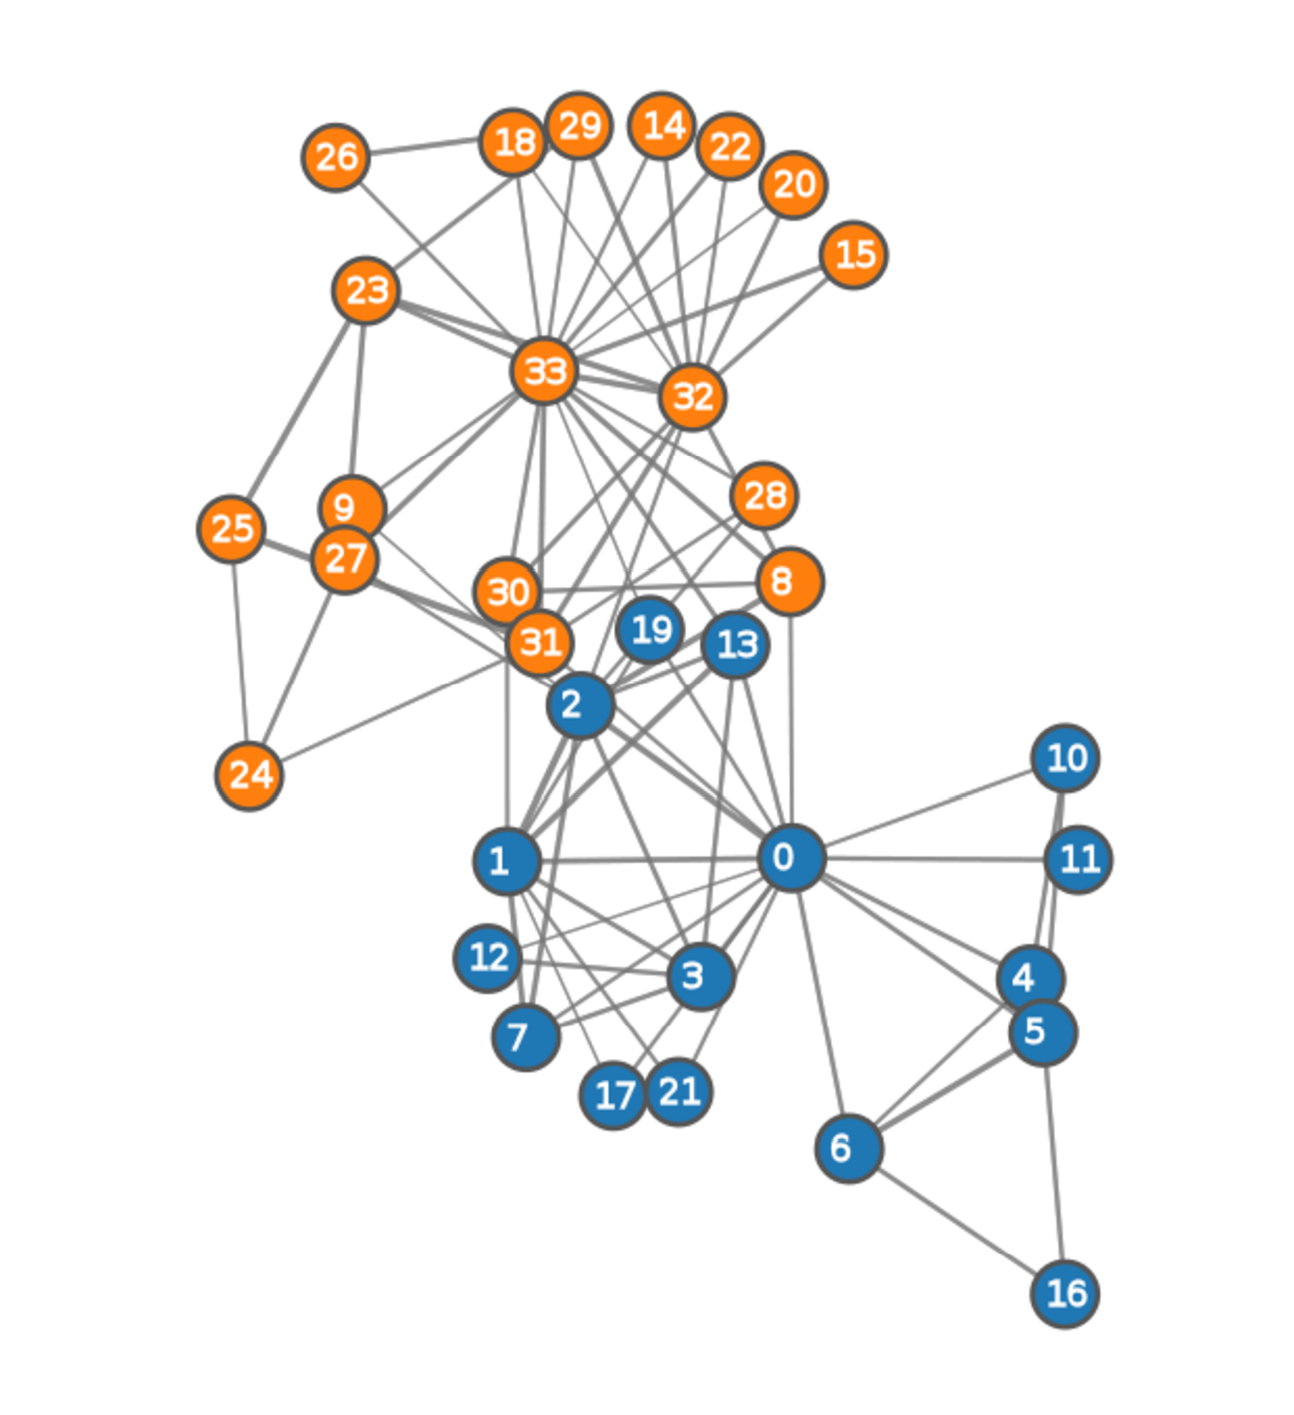
\includegraphics[scale=0.4]{q3/init_graph.pdf}}
\caption{Initial Graph}
\label{fig:init_graph}
\end{figure}

\begin{figure}[h!]
\centering
\fbox{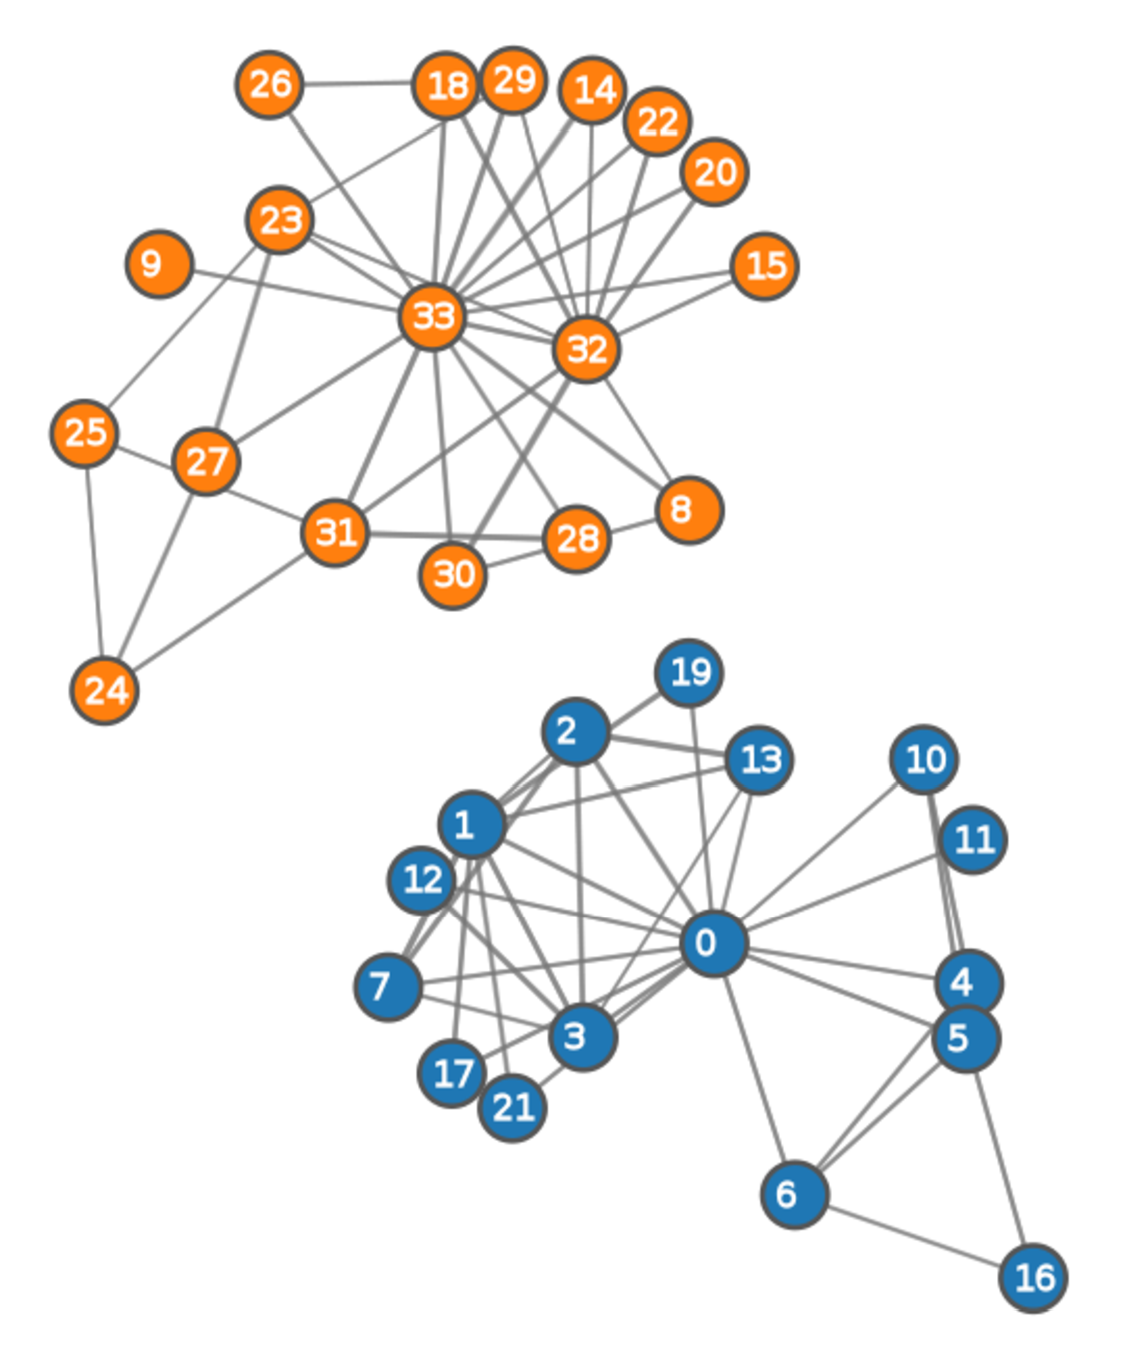
\includegraphics[scale=0.4]{q3/split_graph.pdf}}
\caption{Graph After Split}
\label{fig:split_graph}
\end{figure}

\clearpage

The dataset was first parsed into matrices using the {\tt build\_matrix} function, shown in Listing \ref{listing:convert}. These matrices were converted into python dictionary objects, which are pickled \cite{py:pickle} into the json format \cite{json}. This output was used as the input for the JavaScript code, which uses the D3 library \cite{d3} to create the graphs.

The python code to produce the json data is shown in Listing \ref{listing:convert}.

\lstinputlisting[language=Python, caption={Data Converter}, label=listing:convert]{q3/convert.py}

\clearpage

The JavaScript code to produce the graph is shown in Listing \ref{listing:build}.

\lstinputlisting[language=JavaScript, caption={Building the Graph}, label=listing:build,linerange={27-97},firstnumber=27]{q3/build_graph.html}
